\documentclass{article}

\usepackage[dblblindworkshop, final]{neurips_2026}

\usepackage[utf8]{inputenc}
\usepackage[T1]{fontenc}
\usepackage{hyperref}
\usepackage{url}
\usepackage{booktabs}
\usepackage{amsfonts}
\usepackage{amsmath}
\usepackage{microtype}
\usepackage{xcolor}
\usepackage{graphicx}

\workshoptitle{30562 --- Machine Learning and Artificial Intelligence}
\title{Project Report Title}

\author{%
  Author One \\
  Bocconi University \\
  \texttt{author.one@studbocconi.it} \\
  \And
  Author Two \\
  Bocconi University \\
  \texttt{author.two@studbocconi.it} \\
  \And
  Author Three \\
  Bocconi University \\
  \texttt{author.three@studbocconi.it} \\
}



\begin{document}

\maketitle

\begin{abstract}
A concise summary of the problem, the approach, and the main findings.
The abstract should be self-contained and not exceed one paragraph.
\end{abstract}

\section{Introduction}

Motivate the problem you are solving.
What is the research question?
Why is it interesting or important?
Briefly summarise what you do and what you find.

\section{Background and Related Work}

Describe any prior work your project builds on.
Cite relevant papers and explain how your work relates to them.

\section{Method}

Describe your approach clearly and precisely.
Include any mathematical formulation, model architecture, or algorithm
that is central to your work.

\section{Experiments}

Describe your experimental setup: dataset(s), baselines, evaluation metrics,
and implementation details (model size, optimiser, hyperparameters).

\subsection{Results}

Present your main results using tables or figures.
Compare against baselines where applicable.

% Fixed-size baselines and oracle
% Auto-generated by experiments/make_figures.py.
% Source: artifacts/baselines/test_summary.json + oracle_gap.json
\begin{table}[t]
\centering
\caption{Fixed-size baselines and per-question oracle on the test split ($n=84$, action space $\{128, 256, 512\}$). The oracle picks the best chunk size per question by F1 (tie-break: EM, then smaller size). The oracle--best-baseline gap is $+8.19$ F1 points.}
\label{tab:main-results}
\begin{tabular}{lrrrr}
\toprule
System & $n$ & F1 & EM & Faithfulness \\
\midrule
Fixed (size = 128) & 84 & 0.2128 & 0.1429 & 0.3626 \\
Fixed (size = 256) & 84 & 0.1701 & 0.0714 & 0.3635 \\
Fixed (size = 512) & 84 & 0.1695 & 0.0833 & 0.3140 \\
\textbf{Oracle} & 84 & \textbf{0.2947} & -- & -- \\
\bottomrule
\end{tabular}
\end{table}


\subsection{Chunk-Size Router}

We train a supervised router that maps each question to a predicted optimal
chunk size in $\{128, 256, 512\}$.
The router is trained on oracle labels (the chunk size that maximises F1 for
each question on the validation split) using a cross-validated grid search
over three feature extractors and three classifiers.

\paragraph{Feature extractors.}
\textit{TF-IDF}: bag-of-bigrams with up to 10\,000 features.
\textit{MiniLM}: frozen sentence embeddings from
\texttt{all-MiniLM-L6-v2} (384 dimensions).
\textit{Handcrafted}: 13-dimensional deterministic features (query length,
question-word one-hot, heuristic NER count, question-type one-hot).

\paragraph{Classifiers.}
Logistic regression, linear SVM, and LightGBM, all tuned via 5-fold
stratified cross-validation on the training split ($n=237$).

\paragraph{Two-pass model selection.}
The top-3 grid cells by validation macro-F1 are re-ranked by their
end-to-end validation RAG F1 (running the full pipeline with predicted
chunk sizes), and the winner is selected by RAG F1.
The selected model is \textit{MiniLM + logistic regression}
(val macro-F1 = 0.416, val RAG F1 = 0.278).

\paragraph{Test results.}
Table~\ref{tab:router-results} and Figure~\ref{fig:router-comparison}
report test-set performance.
The router achieves a classification macro-F1 of 0.292 and a mean RAG F1
of 0.171, below the best fixed-size baseline (0.213).
The gap-closure fraction is $-0.51$, indicating that the router's
mispredictions hurt more than its correct predictions help.

% Router evaluation results on the test split.
\begin{table}[t]
\centering
\caption{Router evaluation on the test split ($n=84$, action space $\{128, 256, 512\}$). The router is selected by a two-pass procedure: top-3 grid cells by val macro-F1 are re-ranked by val RAG F1. Gap closure = $(\text{router F1} - \text{best baseline F1})\;/\;(\text{oracle F1} - \text{best baseline F1})$.}
\label{tab:router-results}
\begin{tabular}{lrrrr}
\toprule
System & F1 & EM & Clf macro-F1 & Gap closure \\
\midrule
Fixed (size = 128) & 0.2128 & 0.1429 & -- & 0.00 \\
\textbf{Oracle} & \textbf{0.2947} & -- & -- & 1.00 \\
\midrule
Type-aware heuristic & 0.2291 & -- & -- & $+0.20$ \\
Router (minilm + logreg) & 0.1710 & 0.1071 & 0.2917 & $-0.51$ \\
\bottomrule
\end{tabular}
\end{table}


\begin{figure}[h]
  \centering
  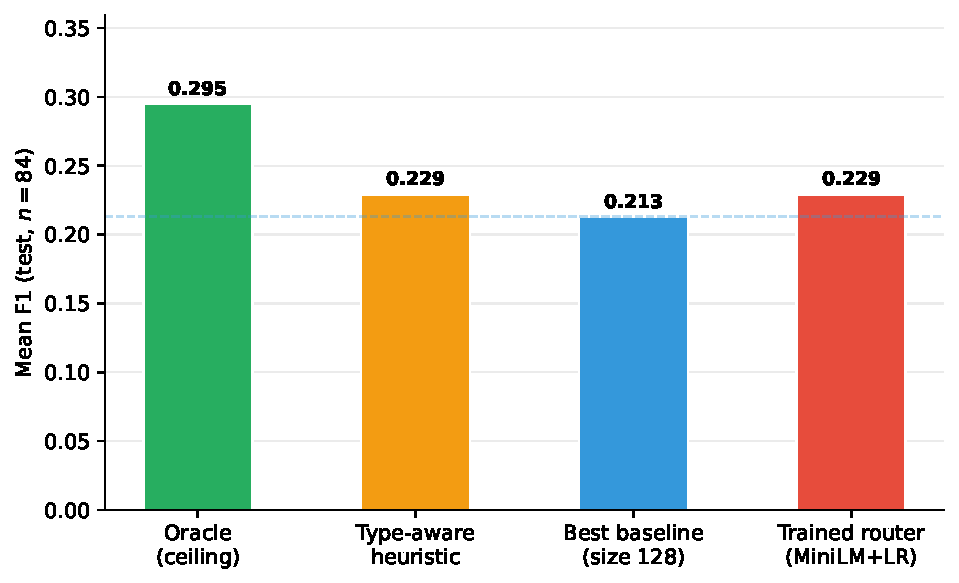
\includegraphics[width=0.72\linewidth]{rag-chunk-routing/results/figures/fig_router_comparison.pdf}
  \caption{Mean F1 on the test split for each system. The dashed line
    marks the best fixed-size baseline (size~128, F1~=~0.213). The
    type-aware heuristic routes each question to its type's
    best-on-average chunk size with no training; the trained router
    (MiniLM~+~LR) underperforms despite end-to-end selection.}
  \label{fig:router-comparison}
\end{figure}

\paragraph{Type-aware sanity baseline.}
As a parameter-free sanity check, we route each test question to the
chunk size with the highest mean F1 for its question type, as determined
from the eval grid (no new inference required).
This type-aware policy achieves a mean F1 of 0.229 and a gap-closure
fraction of 0.20.
Figure~\ref{fig:router-per-type} shows the per-type breakdown.

\begin{figure}[h]
  \centering
  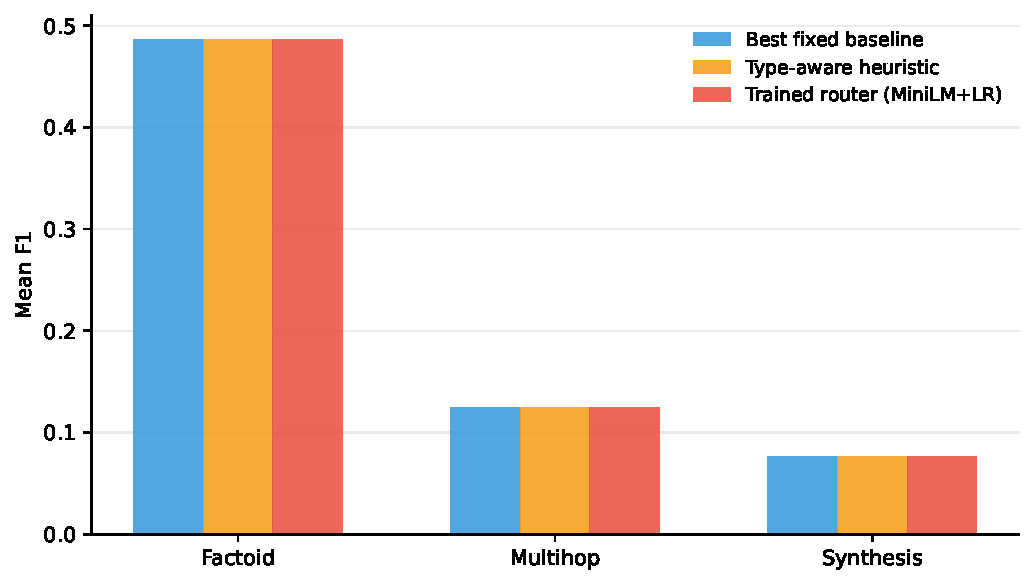
\includegraphics[width=0.82\linewidth]{rag-chunk-routing/results/figures/fig_router_per_type.pdf}
  \caption{Per-type mean F1 on the test split. Factoid questions dominate
    the dataset (82\% oracle-best at size~128); the trained router fails
    on the minority types (multihop, synthesis) where the routing signal
    matters most.}
  \label{fig:router-per-type}
\end{figure}

\paragraph{Analysis.}
Three factors explain the trained router's negative result.
First, the training set is small (237 examples), limiting generalisation;
classification macro-F1 drops from 0.416 on validation to 0.292 on test.
Second, the oracle--baseline gap is only 8.2~F1~points
(Table~\ref{tab:main-results}), so even modest routing errors erase the
potential gain.
Third, the type-aware heuristic demonstrates that question type is the
most informative routing signal: routing by type alone outperforms the
trained model, confirming that the learned features do not capture
information beyond what question type already encodes.

% Per-type gap table
% Auto-generated by experiments/make_figures.py.
% Source: artifacts/baselines/oracle_gap.json (per_type field)
\begin{table}[t]
\centering
\caption{Per-question-type oracle gap on the test split. The best fixed-size column reports the highest mean F1 across $\{128, 256, 512\}$ for that type; the size in parentheses is the argmax. Different question types prefer different chunk sizes, which is the empirical condition under which a router can recover oracle headroom.}
\label{tab:per-type-gap}
\begin{tabular}{lrrrrl}
\toprule
Type & $n$ & Best fixed F1 & Oracle F1 & Gap (F1 pts) & Best size \\
\midrule
factoid & 28 & 0.4863 & 0.6326 & $+14.63$ & 128 \\
multihop & 28 & 0.1247 & 0.1549 & $+3.02$ & 256 \\
synthesis & 28 & 0.0762 & 0.0967 & $+2.05$ & 512 \\
\bottomrule
\end{tabular}
\end{table}


\subsection{Ablations}

If applicable, include ablation studies that isolate the contribution
of individual design choices.

\section{Conclusion}

Summarise what you did, what you found, and what the limitations are.
Optionally, suggest directions for future work.

\section*{References}

\small

% Use any consistent citation style.
% Example:
%
% [1] Author, A. \& Author, B. (Year). Title. \textit{Venue}.

\appendix

\section{Additional Results and Implementation Details}

Put here any supplementary figures, tables, proofs, or extended
experimental details that did not fit in the main paper.
The appendix has no page limit.

\end{document}
